\clearpage
\begin{flushright}
	\textit{Лекция №16}
	\textit{2015.11.10}
\end{flushright}

В прошлой лекции была ошибка. Надо так:
\begin{figure}[H]
    \centering
    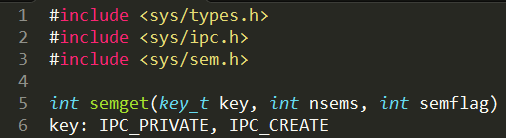
\includegraphics[width=\textwidth]{listing/1.png}
    \caption{listing}
    \label{listing:semget}
\end{figure}

\ref{listing:semget} возвращает идентификатор, и его передаем системному вызову semop()

\section{Программные каналы}

Неименованный – файловой системе не виден, но для него создается дескриптор, который наследуется процессами потомками. В результате процессы родственники могут обмениваться сообщениями. Программный канал буферизуется на трех уровнях (В системной области памяти, но если память заполнена, то наиболее старые буфера отправляются на диск. Если больше 4096 байт, то он будет заблокирован)

\verb|mknode(name, IFFIFO | ACCESS, 0);|\\
\verb|ACCESS| должно быть определено, например 0666

\begin{lstlisting}[language=c, caption = Создание канала, label = listing:create_channel]
# ls | ws -1
\end{lstlisting}

в результате \ref{listing:create_channel} создается канал. Если программный канал не может быть создан, нам возвратят -1. В своих программах нужно проверять.

\section{Сегменты разделяемой памяти}

Особенность в том, что данное системное средство взаимодействия процессов, позволяет множеству процессов отображать системное адресной пространство выделенное под разделяемый сегмент на своё адресное пространство, т.е. созданный разделяемый сегмент подключается с помощью указателя к виртуальному адресному пространству процесса. РП была реализована как средство повышения производительнсоти при обработки сообщений, как универсальное средство в силу того, что разделяемый сегмент подключается ???, при записи сообщения в  разделяемый сегмент и при чтении – копирование не выполняется. Так данное средство позволяет осуществить обмен сообщениями быстро, но РП не имеет средств взаимоисключения. Поэтому РП используеются совместно с семафрами. В адресном простарнстве ядра имеется таблица разделяемых сегментов (= РП). 

\begin{figure}[H]
    \centering
    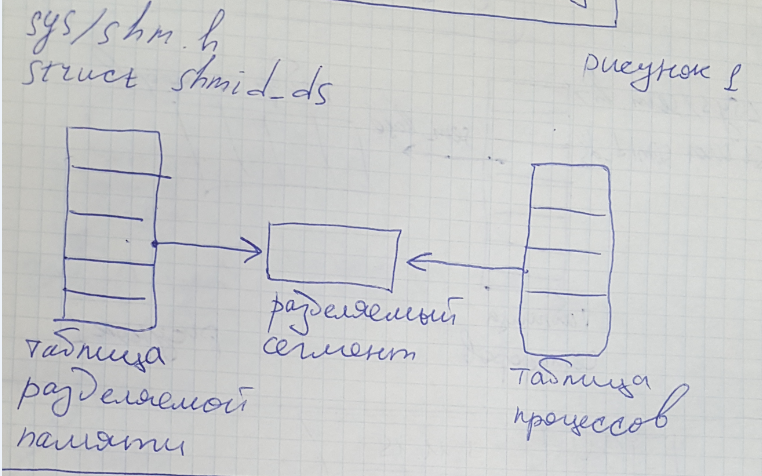
\includegraphics[width=\textwidth]{pic/1.png}
    \caption{pic}
\end{figure}

Процессы, дескрипторы которых в таблице процессов, получают указатель на разделяемый сегмент ???.
\verb|shmget();|

Изменить параметры созданного разд cегмента поможет \verb|shmctl();|\\ 
\verb|shmat()| \verb|shmdt()| - ???.

\begin{figure}[H]
    \centering
    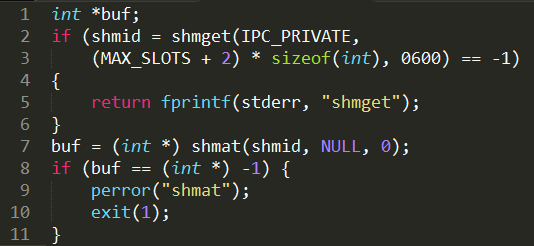
\includegraphics[width=\textwidth]{listing/2.png}
    \caption{listing}
\end{figure}

\begin{figure}[H]
    \centering
    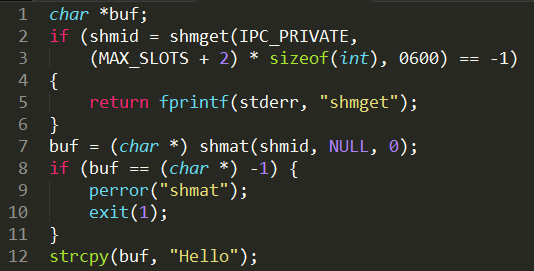
\includegraphics[width=\textwidth]{listing/3.png}
    \caption{listing}
\end{figure}

\begin{table}[H]
\caption{В системе есть ограничения на создание РП}
\begin{tabular}{|l|p{11cm}|}
\hline
Системное ограничение & значение \\
\hline
SHMMNI & Максимальное число разделяемых сегментов, которые могут существовать одновременно \\
\hline
SHMMIN & Минимальный размер разделяемой области памяти в байтах\\
\hline
SHMMAX & \\
\hline
\end{tabular}
\end{table}

\section{Очереди сообщений}

У pipe должен быть и читатель и писатель. Сложные правила взятия сообщения из очереди. Система поддерживает системную таблицу очередей сообщений. 

\begin{figure}[H]
    \centering
    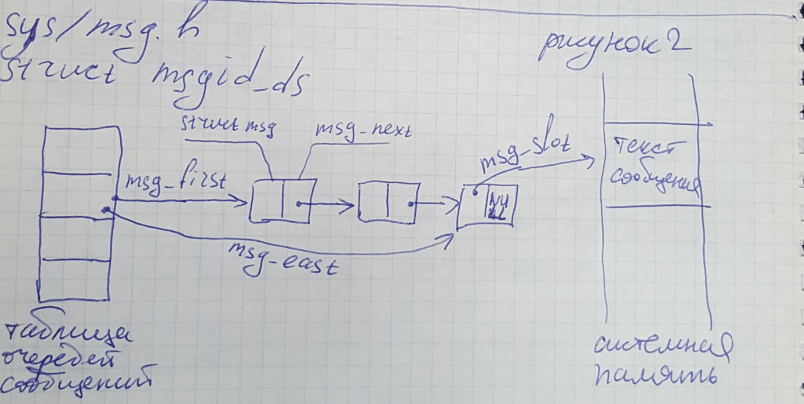
\includegraphics[width=\textwidth]{pic/2.png}
    \caption{pic}
\end{figure}

Когда процесс передает сообщение в очередь, ядро создает для него новую запись и помещает её в конец связного списка записей соответствующих сообщением указанной очереди. В каждой такой записи указывается тип сообщения, размер в байтах, указатель на область данных ядра системы, в которой фактически находится сообщение. Ядро копирует сообщение из пространства отправителя в область данных ядра системы, после чего процесс отправитель может завершиться. Сообщение останется доступным для чтения другим процессам. Когда какой либо процесс выбирает сообщение из очереди, ядро копирует его в адресное пространство этого процесса, после чего запись удаляется (сообщение - потребляемый ресурс, когда получено – перестает существовать). 

Процесс может выбрать сообщение из очереди несколькими способами:
\begin{enumerate}
    \item Взять самое старое сообщение, независимо от его типа.
    \item Если идентификатор сообщения совпадает с идентификатором, который указал процесс. Если существует несколько сообщений с таким идентификатором, то берется самое старое. (идентификатор = тип)
    \item Выбрать сообщение, числовое значение типа которого ??? меньшее или равное значению типа, указанному процессом. 
\end{enumerate} 

Самое главное, процесс, отправивший сообщение, может завершиться. Процесс, заинтересованный в получении сообщения, может взять его несколькими способами, Он может гибко действовать с сообщениями и он не будет блокирован. Так , если вернуться к диаграмме трех состояний блокировки процесса при передачи сообщений, используя очередь сообщений, мы можем избавить процесс от блокировок. Но цена – получаем не то, что нужно, ???.

\begin{figure}[H]
    \centering
    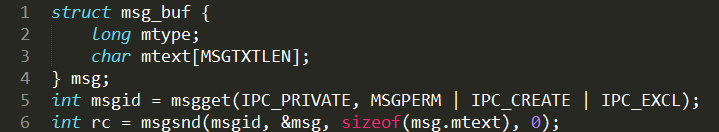
\includegraphics[width=\textwidth]{listing/4.png}
    \caption{listing}
\end{figure}

Windows поддерживает разделяемые сегменты. Определены файлы, отображаемые в память, и установкой параметров можно регламентировать его как РП.  Файлы отображаемые в память позволяют отображать адресное пространство в оперативную память. Для того, чтобы избавиться от области свопинга. Windows поддерживает POSIX.

\chapter{Синхронизация в распределенных системах}

Рассмотрим работы программы make ОС UNIX. В Unix большие программы разбиваются на несколько файлов. Очевидно, что изменения, вносимые в один файл, ??? компиляция только этого файла. Программа make проверяет время последней модификации всех исходных файлов и всех объектных файлов программы. Если исходный файл имеет время последней модификации больше, чем время последней модикации объектного соответствующего файла, то make считает, что он был изменен и перекомпилирует его. 
Рассмотрим ситуацию в распределённой системе. Есть несколько компов. На одном мы редактируем, на другом – перекомпилируем.

\begin{figure}[H]
    \centering
    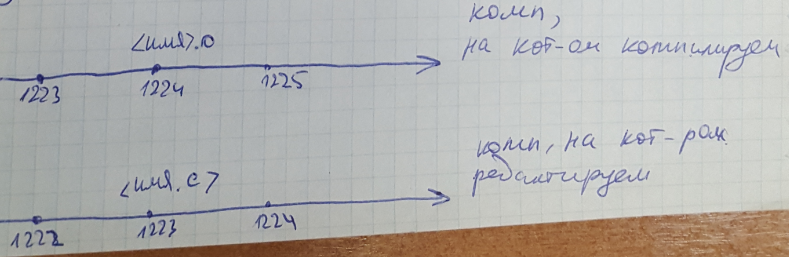
\includegraphics[width=\textwidth]{pic/3.png}
    \caption{pic}
\end{figure}

Связанно с локальными часами. На компах кварцевые генераторы. Любое техническое устройство имеет определенные характеристики, в том числе кварцевый генератор имеет допустимую ошибку генерации тиков. Погрешность – $10^{-5}$. Если таймер генерирует 60 прерываний / секунду, то в час он сгенерирует 216 000 тиков, конкретная машина может выдать значения тиков в следующем диапазоне: 215996 – 216002 за час. Вывод – не можем синхронизироваться по локальным часам. 